%!TEX root = ../report.tex
%*******************************************************************************
%                       Design & technical specifications                      %
%*******************************************************************************


\chapter{Design \& technical specifications}


\section{Introduction}
    Once the system requirements are identified, the next step would be to prepare the conceptual representation
    of the project. This part focuses just on the worker, going all the way from its mission and details of
    communication with the scheduler to the energy consumption part.

\section{Desing and architecture}

    \begin{figure}[!h]\centering
        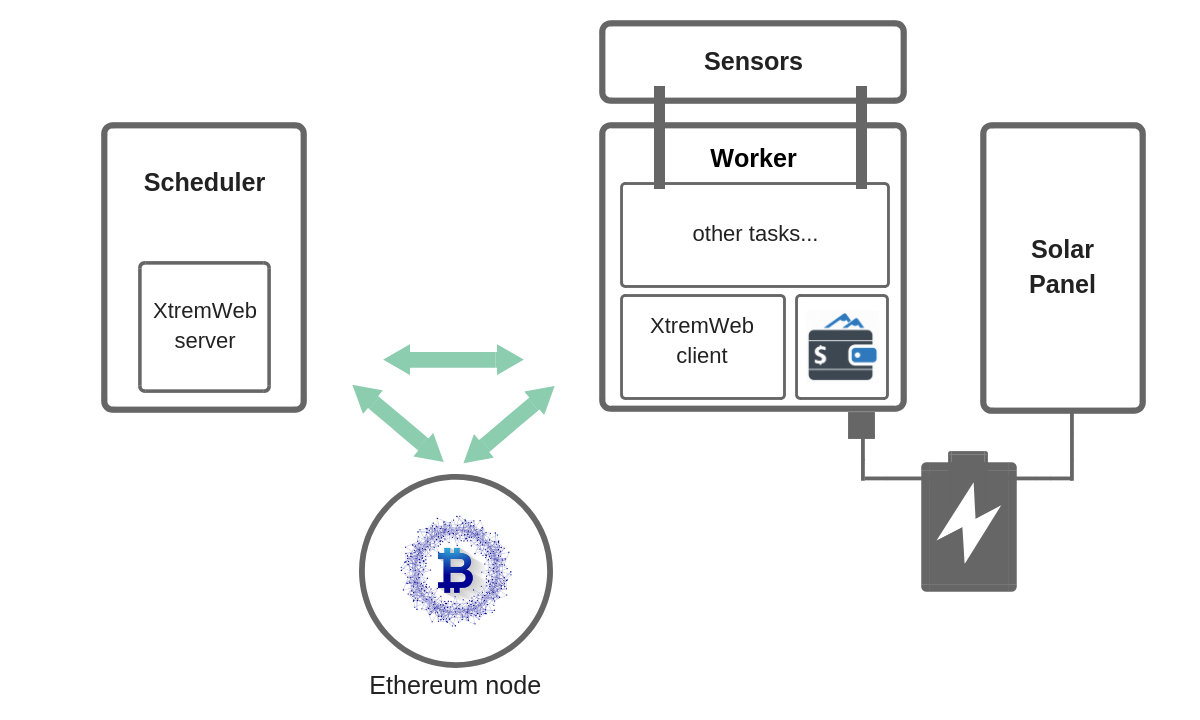
\includegraphics[width=.9\columnwidth]{5-Design/figs/worker-diagram.png}
        \caption{xxxxxxxxxx}
    \end{figure}

    \subsection{xtremweb}
    \subsection{blockchain}
    \subsection{energy}
    \subsection{IoT}

    talk about the diagram
    
    blockchain: wallet using sdk --> ansible to verify
    
    xtremweb: add arm support

    cluster --> swarm
    
    Energy: solar panel, battery, voltage, watts, hours board consumption --> tests

    challenges: x-compiling --> Qemu, optimize docker image size --> cache best practices, specs --> heap size
    
    develop dapps: names

    docker(optimisation) java shell 

\section{Energy}

\section{Geth node}

\section{Use cases}
    \subsection{Surveillance Camera}
    \subsection{Weather Station}


\section{Technical Specifications}
    \subsection{specs of the board}
    \subsection{automate configuration and deployment}
    \subsection{develop dapps (use cases)}
    \subsection{deployment of all the environment}
    \subsection{cross-compiling}
    \subsection{cluster}


\section{Conclusion}